% !TeX program = xelatex
% !TeX encoding = UTF-8

\documentclass[timesfont,no-math]{JXUSTmodeling}%设置默认英文字体为Times New Roman,但不改变数学字体设置
%\documentclass[timesfont,no-math,bwprint]{JXUSTmodeling}%取消彩色,只使用黑色文本

%\bibliographystyle{plain}
\renewcommand*{\lstlistingname}{代码}

\title{江西理工大学数学建模 \LaTeX{} 模板}%设置标题


\authorone{队员1}%队员 1 姓名
\authoroneclass{专业1}%队员 1 专业
\authortwo{队员2}%队员 2 姓名
\authortwoclass{专业2}%队员 2 专业
\authorthree{队员3}%队员 3 姓名
\authorthreeclass{专业3}%队员 3 专业
\logo{logo.jpg}% logo 标志

\usepackage{hologo}
\usepackage{lipsum}

\begin{document}

	\maketitle%生成标题页

	\newpage
	\vspace*{\stretch{1}}
	\begin{figure}[!ht]
		\centering
		\heiti\zihao{2} {\color{red}郑重声明}
		
		本模板不提供任何保证. 
		
		您使用本模板造成的任何后果与作者无关.
		
		本模板不用于任何商业目的.
		
		如果是非商业目的,您可以以任意方式使用本模板而无需通知作者.
		
		但如果是商业目的,请{\color{red}重新阅读}此郑重申明.
	\end{figure}
	\vspace*{\stretch{1}}
\thispagestyle{empty}
	
	
	\newpage
	\phantomsection
	\addcontentsline{toc}{section}{摘\hspace{2em}要}
	\section*{摘\hspace{2em}要}%摘要页
	{\zihao{4} 本项目已上传至 GitHub, 你可以在 \url{https://github.com/sikouhjw/LaTeX-learning-notes} 获取最新的版本, 或者告知我们你的建议.}
	
	\vspace{1em}
	
	更新说明: 此次更新设置了添加了文档类选项 timesfont 和 bwprint, 使用 timesfont 选项将设置默认英文字体为 Times New Roman, 使用 
	 bwprint 选项将全局使用黑色文本. 另外添加了可以直接使用的 matlab 和 python 代码环境, 将摘要和参考文献添加到书签中, 
	虽然基本的格式都已由 \LaTeX{} 自动完成, 但是各种细致的调整仍需同学们手动进行.
	
	\noindent\rule{\textwidth}{1pt}

	本模板是为江西理工大学数学建模竞赛准备的. 为了让写作的同学们把更多精力放在写作的内容上, 
	而不是论文的格式上, 我编写了这个模板. 要使用本模板的同学应该要阅读过 lshort-zh \cite{lshort-zh} 的大部分内容,
	会使用 \LaTeX{} 的基本命令, 能够用 \LaTeX{} 编写自己的文档.
	
	务必使用 UTF8 编码和 \texttt{xelatex} 命令编译本模板.
	
	此模板示例在 win10 系统 和 \TeX\,Live2018 下可以正常运行.
	
	本模板使用 ctexart 文档类\cite{ctex-package}修改了文档标题的基本格式和行距, 使用 geometry 宏包设置页边距, 
	重定义 \verb|\maketitle|\cite{classes} 命令改变了封面的样式, 参考了全国大学生数学建模模板\cite{CUMCMThesis}的
	样式, 使之符合江西理工大学数学建模竞赛论文格式规范中的要求.
	
	本模板并未使用 \hologo{BibTeX} 作为参考文献的排版工具, 其中有作者水平有限的原因, 但更多的是因为考虑到同学们要引用的参考文献
	大多数都是中文书籍. 而就作者了解, 能够完整导出 \hologo{BibTeX} 数据的中文书籍较少, 另外知网不能够导出 \hologo{BibTeX} 数据.
	所以本模板不使用 \hologo{BibTeX} 排版参考文献. 如果同学们真的要要使用 \hologo{BibTeX} 排版参考文献, 可以将导言区中的
	\verb|\bibliographystyle{plain}| 和 \verb|thebibliography| 环境前的 \verb|\bibliography{reference}| 取消注释, 并且
	注释掉 \verb|thebibliography| 环境, 将 \hologo{BibTeX} 数据导入 reference.bib 文件中\footnote{此过程无先后顺序之分.},
	这样就可以使用 \hologo{BibTeX} 排版参考文献.
	
	本模板用 listings 宏包\cite{listings-package}定制了代码环境, 默认语法高亮的颜色设置与 Matlab 的默认设置一致,
	但是并未设置代码为 Matlab 代码, 需要同学们手动设置代码类型\footnote{\LaTeX{} 默认的 Matlab 关键词与 Matlab 默认的 Matlab 关键词不同, 如果需要实现和 Matlab 默认一样的效果, 需要额外调整, 调整方法见 \href{JXUSTmodeling.cls}{JXUSTmodeling.cls}.}, 
	设置实例见附录~\ref{app:2} 代码~\ref{lst:1}.
	
	表格推荐使用三线式表格,用 \verb|\toprule| 画表格顶部的水平线,
	用 \verb|\midrule| 和 \lstinline[basicstyle=\ttfamily]|\cmidrule{column1-column2}| 画表格中间的水平线, 用 \verb|\bottomrule| 画
	表格底部的水平线. 示例代码见附录~\ref{app:2} 代码~\ref{lst:tab},
	示例输出结果见附录~\ref{app:2} 表~\ref{tab:feature}.
	
	虽然基本的格式都已由 \LaTeX{} 自动完成, 但是各种细致的调整仍需同学们手动进行. 
	
	更多说明见源文件注释.

	
	\setcounter{page}{1}%设置页码为1
	\noindent {\bfseries 关键词}\quad 江西理工大学 \quad \LaTeX{}\quad 数学建模 \quad 
	\newpage
	\section*{举个例子}
	比较一下 \LaTeX{} 和 word 的数学公式效果:
	\newtheorem*{thm}{Theorem}
	
	\begin{thm}[Newton-Leibniz formula]
	若函数 $f(x)$ 在区间 $[a,b]$ 连续, 且 $F(x)$ 是$f(x)$ 的原函数, 则
	\[
		\int_a^b f(x) \dd x= F(b) - F(a) .
	\]
	\end{thm}
	上式是 \LaTeX{} 的数学公式效果, word 的数学公式效果如下图
	\begin{center}
	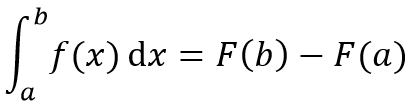
\includegraphics[width=50mm]{BasicTheoremOfCalculus.png}
	\end{center}
	
	
	\section{问题的提出}\label{sec:1}
	校级数学建模竞赛即将开始, 数学建模分为三个部分: 建模, 计算, 写作. 其中每个部分都十分重要, 
	写作工具的选择也十分重要. 我们应该选择适合自己, 并且容易使用的写作工具. 
	目前的主流写作工具应该是 word, 而学术论文写作一般使用 \TeX{} 发行版. 这两者都可以用于数学建模的写作.
	这两种工具都有各自的优缺点, \LaTeX{} 相对于 word 的优缺点\cite{lshort-zh} 的粗略描述见表~\ref{tab:feature}.
	
	
	问题 1: 同学们应该使用哪种写作工具?
	
	……
	
	……
	
	填充文本
	
	\lipsum[1-2]
	
	
	\section{问题的分析}\label{sec:2}
	问题 1 分析: 这个问题应该结合写作工具的特点和写作同学对各种写作工具的熟悉程度来决定.
	
	……
	
	……
	
	填充文本
	
	\lipsum[3-4]
	
	\section{模型的假设和符号说明}\label{sec:3}
	\subsection{模型的假设} \label{ssec:3.1}
	\begin{enumerate}
		\item 假设同学们对 word 和 \LaTeX{} 都有所了解.
		\item 假设同学们对论文的要求和愿意用来学习\LaTeX 的精力都是一样的.
		\item ……
		
		\noindent\makebox[0em][c]{……}
	\end{enumerate}
	\subsection{符号说明}\label{ssec:3.2}
	见表~\ref{tab:symbol}
	
	\begin{table}
		\centering
		\caption{符号说明}\label{tab:symbol}
		\begin{tabularx}{0.8\textwidth}{YY}
			\toprule
			符号		&		说明		\\
			\midrule
			\LaTeX		&	最广泛应用的一种格式	\\
			\midrule	
			\hologo{XeTeX}	&	排版引擎	\\
			\midrule		
			\hologo{pdfTeX}	&	排版引擎	\\
			\midrule
			\texttt{xelatex}	&	命令		\\
			\midrule
			\texttt{pdflatex}		&		命令		\\
			\midrule
			……			&		……				\\
			\bottomrule
		\end{tabularx}
	\end{table}
	填充文本
	
	\lipsum[5-6]
	
	\section{模型的建立与求解}\label{sec:4}
	对于问题 1 ,我们……
	
	填充文本
	
	\lipsum[7-8]
	\section{模型的检验}\label{sec:5}
	结果与实际比较……
	
	填充文本
	
	\lipsum[9-10]
	
	\section{模型的评价与改进}\label{sec:6}
	虽然这个模型解决了……
	
	填充文本
	
	\lipsum[11-12]
	
	 \phantomsection
	 \addcontentsline{toc}{section}{\refname}
	\begin{thebibliography}{99}
		\bibitem{lshort-zh} China\TeX{} 论坛, 《 一份不太简短的 \LaTeXe{} 介绍》 (lshort-zh).
		\bibitem{ctex-package} \CTeX.ORG,《\CTeX{} 宏集手册》.
		\bibitem{classes}	Leslie Lamport, Frank Mittelbach, Johannes Braams, 《Standard Document 
		Classes for \LaTeX{} version 2e${}^*$》.
		\bibitem{CUMCMThesis} \href{www.latexstudio.net}{\LaTeX{} 科技排版工作室}, 《 全国大学生数学建模竞赛编写的 \LaTeX 模板》.
		\bibitem{listings-package} Carsten Heinz, Brooks Moses, Jobst Hoffmann, 《 The Listings Package》.
	\end{thebibliography}
	\appendix
	
	\vfill

	\section{Matlab 程序}\label{app:1}
	\begin{matlab}
	clc,clear,close
	t=0:0.1:20;
	r=exp(-0.2*t);
	th=0.5*pi*t;
	x=r.*cos(th);
	y=r.*sin(th);
	z=sqrt(t);
	subplot(1,2,1)
	plot3(x,y,z);
	title('螺旋线');
	text(x(end),y(end),z(end),'终点');
	xlabel('\it X=\rm e^{-0.2\it t}\rm cos(\pi\it t)');
	ylabel('Y轴');zlabel('Z轴');
	subplot(1,2,2);
	plot3(x,y,z);
	axis([-1,1,-1,1,0,4]);
	grid on;
	\end{matlab}
	\vfill
	\clearpage
	
	\section{Python 程序}\label{app:3}
	\begin{python}
	for i in range(3):
		print('The cover is not so good that I think we should redefine it!')
	print('We have no ability to do it! We need help!')
	\end{python}
	
	\section{\LaTeX{} 程序}\label{app:2}
	\subsection{lstlisting 示例}
	\begin{figure*}[!htbp]
		\centering
	\begin{lstlisting}[language={[LaTeX]TeX},caption={\LaTeX{} 代码实例},label={lst:1},escapechar=\%]
\begin{lstlisting}[language={[LaTeX]TeX},caption={\LaTeX{} 代码},label={lst:2}]
	\begin{figure}[!htbp]
		\centering\kaishu
		春江花月夜~~张若虚\\
		春江潮水连海平,海上明月共潮生。\\
		滟滟随波千万里,何处春江无月明!\\
		江流宛转绕芳甸,月照花林皆似霰。\\
		空里流霜不觉飞,汀上白沙看不见。\\
		江天一色无纤尘,皎皎空中孤月轮。\\
		江畔何人初见月?江月何年初照人?\\
		人生代代无穷已,江月年年望相似。\\
		不知江月待何人,但见长江送流水。\\
		白云一片去悠悠,青枫浦上不胜愁。\\
		谁家今夜扁舟子?何处相思明月楼?\\
		可怜楼上月徘徊,应照离人妆镜台。\\
		玉户帘中卷不去,捣衣砧上拂还来。\\
		此时相望不相闻,愿逐月华流照君。\\
		鸿雁长飞光不度,鱼龙潜跃水成文。\\
		昨夜闲潭梦落花,可怜春半不还家。\\
		江水流春去欲尽,江潭落月复西斜。\\
		斜月沉沉藏海雾,碣石潇湘无限路。\\
		不知乘月几人归,落月摇情满江树。\\
	\end{figure}
\end
	\end{lstlisting}
		如果在本模板中运行代码~\ref{lst:1}, 将会得到代码~\ref{lst:2}.
	\end{figure*}
	\begin{figure*}[!htbp]
		\centering
		\begin{lstlisting}[language={[LaTeX]TeX},caption={\LaTeX{} 代码},label={lst:2}]
	\begin{figure}[!htbp]
		\centering\kaishu
				春江花月夜~~张若虚\\
		春江潮水连海平,海上明月共潮生。\\
		滟滟随波千万里,何处春江无月明!\\
		江流宛转绕芳甸,月照花林皆似霰。\\
		空里流霜不觉飞,汀上白沙看不见。\\
		江天一色无纤尘,皎皎空中孤月轮。\\
		江畔何人初见月?江月何年初照人?\\
		人生代代无穷已,江月年年望相似。\\
		不知江月待何人,但见长江送流水。\\
		白云一片去悠悠,青枫浦上不胜愁。\\
		谁家今夜扁舟子?何处相思明月楼?\\
		可怜楼上月徘徊,应照离人妆镜台。\\
		玉户帘中卷不去,捣衣砧上拂还来。\\
		此时相望不相闻,愿逐月华流照君。\\
		鸿雁长飞光不度,鱼龙潜跃水成文。\\
		昨夜闲潭梦落花,可怜春半不还家。\\
		江水流春去欲尽,江潭落月复西斜。\\
		斜月沉沉藏海雾,碣石潇湘无限路。\\
		不知乘月几人归,落月摇情满江树。\\
	\end{figure}
		\end{lstlisting}
		如果在本模板中运行代码~\ref{lst:2},则会得到图~\ref{fig:poem}.
	\end{figure*}
	
	\begin{figure}[!htbp]
		\centering\kaishu
				春江花月夜~~张若虚\\
		春江潮水连海平,海上明月共潮生。\\
		滟滟随波千万里,何处春江无月明!\\
		江流宛转绕芳甸,月照花林皆似霰。\\
		空里流霜不觉飞,汀上白沙看不见。\\
		江天一色无纤尘,皎皎空中孤月轮。\\
		江畔何人初见月?江月何年初照人?\\
		人生代代无穷已,江月年年望相似。\\
		不知江月待何人,但见长江送流水。\\
		白云一片去悠悠,青枫浦上不胜愁。\\
		谁家今夜扁舟子?何处相思明月楼?\\
		可怜楼上月徘徊,应照离人妆镜台。\\
		玉户帘中卷不去,捣衣砧上拂还来。\\
		此时相望不相闻,愿逐月华流照君。\\
		鸿雁长飞光不度,鱼龙潜跃水成文。\\
		昨夜闲潭梦落花,可怜春半不还家。\\
		江水流春去欲尽,江潭落月复西斜。\\
		斜月沉沉藏海雾,碣石潇湘无限路。\\
		不知乘月几人归,落月摇情满江树。\\
		\caption{春江花月夜}\label{fig:poem}
	\end{figure}
	\clearpage
	\subsection{三线表示例}
	\begin{lstlisting}[language={[LaTeX]TeX},caption={\LaTeX{} 代码},label={lst:tab}]
	\begin{table}[!htbp]
	\centering
	\caption{\LaTeX{} 相对于 word 的优缺点}\label{tab:feature}
	\begin{tabularx}{0.8\textwidth}{XX}
	\toprule
	优点				&		缺点			\\
	\midrule
	专业的排版输出		&	入门门槛高			\\
	\midrule
	方便而强大的数学公式排版能力,无出其右					&
	排查错误困难										\\
	\midrule
	绝大多数时候,无需(或很少)操心文档的版面设计				&
	样式定制困难								\\
	\midrule
	很容易生成复杂的专业排版元素						&
	为了查看生成的文档,用户总要不停地编译				\\
	\midrule
	\dots\dots			&							\\
	\bottomrule
	\end{tabularx}		
	\end{table}
	\end{lstlisting}
	输出示例见表~\ref{tab:feature}
	
	\begin{table}[!htbp]
		\centering
		\caption{\LaTeX{} 相对于 word 的优缺点}\label{tab:feature}
		\begin{tabularx}{0.8\textwidth}{XX}
			\toprule
			优点				&		缺点			\\
			\midrule
			专业的排版输出		&	入门门槛高			\\
			\midrule
			方便而强大的数学公式排版能力,无出其右					&
			排查错误困难										\\
			\midrule
			绝大多数时候,无需(或很少)操心文档的版面设计				&
			样式定制困难								\\
			\midrule
			很容易生成复杂的专业排版元素						&
			为了查看生成的文档,用户总要不停地编译				\\
			\midrule
			\dots\dots			&							\\
			\bottomrule
		\end{tabularx}		
	\end{table}
\end{document}